% ==============================================================================
% Project Nexus — Academic Whitepaper
% Template: IEEEtran (Two-Column)
% Phase 1: Preamble + Abstract + §1 Introduction
% ==============================================================================
\documentclass[conference,10pt]{IEEEtran}
\IEEEoverridecommandlockouts

% --- Mathematics ---
\usepackage{amsmath,amssymb,amsfonts}
\usepackage[T1]{fontenc}
\usepackage{mathptmx}
\usepackage{microtype}

% --- Tables ---
\usepackage{booktabs}
\usepackage{multirow}
\usepackage{array}
\usepackage{tabularx}

% --- Figures ---
\usepackage{graphicx}
\usepackage{float}

% --- Code Listings ---
\usepackage{listings}
\lstset{
  basicstyle=\ttfamily\footnotesize,
  breaklines=true,
  frame=single,
  language=C++,
  numbers=left,
  numberstyle=\tiny,
  captionpos=b
}

% --- Algorithms ---
\usepackage[ruled,vlined,linesnumbered]{algorithm2e}

% --- Cross-References & Hyperlinks ---
\usepackage[colorlinks=true,citecolor=blue,linkcolor=blue,urlcolor=blue]{hyperref}
\usepackage[capitalise,noabbrev]{cleveref}

% --- Units ---
\usepackage{siunitx}
\sisetup{per-mode=symbol}

% --- Miscellaneous ---
\usepackage{xspace}
\usepackage{balance}

% --- TikZ & Drawings ---
\usepackage{tikz}
\usetikzlibrary{shapes.geometric,arrows.meta,positioning,calc,fit}
\usepackage{pgfplots}
\pgfplotsset{compat=1.18}

% --- Custom Commands ---
\newcommand{\Nexus}{\textsc{Nexus}\xspace}
\newcommand{\atb}{\texttt{.atb}\xspace}
\newcommand{\cmark}{\ding{51}}
\newcommand{\xmark}{\ding{55}}

% ==============================================================================
% DOCUMENT BEGIN
% ==============================================================================
\begin{document}

\title{Nexus: Eliminating Tool Schema Prefill via User-Space KV Cache Memory Mapping in Unified Architectures}

% --- AUTHORS: Mustafa Arslan ---
\author{
  \IEEEauthorblockN{Mustafa Arslan\thanks{Source code available at: \url{https://github.com/mustafarslan/nexus}.}}
  \IEEEauthorblockA{Independent Researcher, Istanbul, Turkiye\\
  mustafarslan35@gmail.com}
}

\maketitle

% ==============================================================================
% ABSTRACT
% ==============================================================================
\begin{abstract}
The Model Context Protocol (MCP) enables large language models (LLMs) to
invoke external tools by appending JSON schema descriptions to the prompt
context window. In multi-tenant agentic deployments, these schemas routinely
span $10^{3}$--$10^{5}$ tokens, imposing a quadratic $\mathcal{O}(N^{2})$
self-attention prefill cost on every invocation turn. We present \Nexus, a
zero-allocation memory management unit (MMU) that bypasses this
prefill bottleneck through three coordinated mechanisms: (1)~an L1 Semantic
Lookaside Buffer (SLB) performing microsecond-scale ($\approx 2.25\,\mu\text{s}$)
SIMD-accelerated INT8 dot-product scans over quantized tool embeddings;
(2)~a Left-Child Right-Sibling (LCRS) radix trie finite-state machine (FSM)
that constrains token generation to valid tool routes using static cache-aligned memory;
and (3)~a stride-aware KV cache splicer that loads pre-compiled tool schemas via
user-space Direct I/O into a pinned arena and blits them into the active attention
context, eliminating redundant attention prefill passes. On an Apple M4~Max under a unified memory
architecture, \Nexus reduces time-to-first-token (TTFT) from
\SI{2226.00}{\milli\second} (FlashAttention-2 GPU prefill of 12,500~tokens)
to \SIrange{10.6}{22.3}{\milli\second} (warm/cold splice P50 on Qwen2.5-14B real KV)---a
\(\approx\!1.64\times\) overhead vs.\ single-schema prefill rather than the
\(145\times\) figure previously reported from synthetic 0.5B microbenchmarks.
End-to-end splice-with-suffix-recompute TTFT is \(\approx\!\SI{1.8}{\second}\) at
P=256; the G4 viability gate fails at P=1024 without high suffix fractions.
Retrieval recall@1 is \(\approx\!0.85\) on gold queries (0.81 on corrected N100/N1000
manifests); 14B listwise rerank reaches 0.94 tool-hit but remains the accuracy bottleneck.
Every component operates without dynamic memory allocation on the critical path.
\end{abstract}

\begin{IEEEkeywords}
Large language models, KV cache management, context routing, memory management
unit, constrained decoding, SIMD, zero-copy KV cache splicing
\end{IEEEkeywords}

% ==============================================================================
% §1  INTRODUCTION
% ==============================================================================
\section{Introduction}
\label{sec:introduction}

The integration of external tools into large language model (LLM) workflows has
extended the operational capabilities of conversational agent architectures.
Frameworks such as the Model Context Protocol (MCP)~\cite{anthropic2024mcp}
standardize how LLMs interact with external APIs: the serving infrastructure
injects complete JSON schema descriptions---specifying function signatures,
parameter types, enumeration constraints, and natural-language
docstrings---directly into the prompt context window before each inference
turn. The model then generates a structured tool invocation conforming to one
of the provided schemas.

However, this schema injection pattern introduces significant computational
overhead during prompt evaluation. The self-attention mechanism in
Transformer-based architectures~\cite{vaswani2017attention} computes pairwise
interactions across all $N$ tokens in the context window, requiring
$\mathcal{O}(N^{2})$ floating-point operations during the prefill phase. In agentic systems supporting multi-domain operations (e.g., file
manipulation, database querying, web search), the combined schema payload
routinely spans $10^{3}$ to $10^{5}$ tokens. For example, evaluating a
12,500-token tool schema block on an Apple M4~Max GPU requires
\SI{2226.00}{\milli\second} (P50 latency), exceeding typical interactive latency
budgets.

\subsection{Limitations of Prefix Caching in Dynamic Workloads}
\label{subsec:naive-caching}

Standard prefix caching~\cite{kwon2023vllm,zheng2024sglang} amortizes prefill
costs by reusing Key-Value (KV) cache blocks of shared prompt prefixes across requests.
However, in dynamically routed agentic workflows, the target tool schema varies
across successive turns (e.g., invoking a file-system tool at step~$t$ and a
database tool at step~$t{+}1$). Because prefix caching requires strict prefix matching starting from position 0, any deviation in the prefix (such as dynamic user queries, conversational history, or intermediate reasoning traces generated prior to the tool block) invalidates the cache for all downstream tokens. In such environments, tool schemas are injected at arbitrary, dynamic branch points. Since these schemas are mutually exclusive yet occupy the identical positional interval, the prompt context diverges at the tool block boundary. This divergence invalidates the cached KV tensors of subsequent tokens, forcing a full quadratic $\mathcal{O}(S^2)$ attention prefill recomputation for the entire schema sequence.

\subsection{The Virtual Memory Analogy}
\label{subsec:vm-analogy}

We identify a structural analogy between LLM tool schema routing and OS virtual memory
management, treating the transformer context window as a virtual address space and
individual tool schemas as independent memory pages managed by a software-based Memory
Management Unit (MMU). In conventional hardware architectures, the MMU coordinates
virtual-to-physical address translation through three mechanisms: a Translation Lookaside
Buffer (TLB) that provides fast, associative caching of active page mappings; a
hierarchical page table walked to resolve address mappings on a TLB miss; and a page
fault handler that transparently swaps pages from secondary storage into physical memory.

While this analogy is an architectural metaphor rather than a strict mapping---notably
because LLM KV caches possess causal position dependencies (Rotary Position Embeddings, or RoPE)
that differentiate them from independent physical memory pages, and the L1 Semantic
Lookaside Buffer (SLB) performs probabilistic semantic similarity scans rather than
deterministic hardware tag matches---\Nexus instantiates this design pattern for LLM
context routing. First, the L1 Semantic Lookaside Buffer (SLB) serves as a semantic
lookaside cache, executing a SIMD-accelerated, INT8-quantized similarity scan
($\approx \SI{2.25}{\micro\second}$) over registered tool embeddings to identify the top-$K$ candidate tool
routes. Second, the Left-Child Right-Sibling (LCRS) Radix Trie FSM maps valid token paths,
acting as a deterministic page table walk that restricts vocabulary generation to valid tool names.
Finally, the KV Cache Splicer behaves as a page fault handler; upon tool resolution, it loads the
pre-compiled tool schema's serialized FP16 KV cache (stored in a binary \atb file) from storage
into a pre-pinned host arena via user-space Direct I/O, then blits it into
physical VRAM with stride-aligned tensor copies and dynamic RoPE shifts.

\subsection{Contributions}
\label{subsec:contributions}

This paper makes the following contributions:

\begin{enumerate}
  \item[\textbf{C1.}] \textbf{Zero-Allocation Semantic Routing:} We design
    and implement an L1 Semantic Lookaside Buffer using INT8 symmetric
    quantization and architecture-specific SIMD kernels (ARM NEON, Intel AVX-VNNI,
    and AVX2) that evaluates tool candidate similarity in \SI{2.25}{\micro\second}.

  \item[\textbf{C2.}] \textbf{Deterministic Constrained Routing:} We
    introduce a Left-Child Right-Sibling radix trie FSM operating on a
    contiguous flat-array arena with per-sequence state isolation
    (\texttt{alignas(128)} matching CPU cache line alignment), achieving lock-free
    logit masking without dynamic heap allocation.

  \item[\textbf{C3.}] \textbf{User-Space KV Cache Splicing:} We implement a
    stride-aware cache splicer loading pre-compiled \texttt{.atb} binaries via user-space
    Direct I/O into a pinned arena, performing 2D memory blitting and dynamic RoPE position
    correction in \SIrange{10.6}{22.3}{\milli\second} on unified memory architectures
    (Qwen2.5-14B real KV; see \texttt{bench\_phase21\_ttft\_real.json}).

  \item[\textbf{C4.}] \textbf{Zero-Allocation C++23 Systems Design:} We contribute
    a zero-allocation task and resource execution system, including cache-line-aligned
    coroutine task dispatch, destructive move semantics, RAII hazard guards with
    ABA protection, and thread-local hysteresis-controlled buffers.
\end{enumerate}

The remainder of this paper is organized as follows. \Cref{sec:related-work}
surveys related work in KV cache management, constrained decoding, and
efficient attention. \Cref{sec:architecture} details the \Nexus three-stage
routing pipeline. \Cref{sec:systems} exposes the low-level C++23 systems
engineering. \Cref{sec:evaluation} presents the experimental evaluation.
\Cref{sec:discussion} discusses limitations and future work.
\Cref{sec:conclusion} concludes.

% ==============================================================================
% §2  RELATED WORK
% ==============================================================================
\section{Related Work}
\label{sec:related-work}

We situate \Nexus within three active research areas: KV cache management for
LLM serving, constrained decoding for structured generation, and efficient
attention mechanisms.

\subsection{KV Cache Management and Disaggregated Serving}
\label{subsec:rw-kvcache}

\textbf{PagedAttention.} Kwon et al.~\cite{kwon2023vllm} introduced
PagedAttention in the vLLM serving system, which partitions the KV cache into
fixed-size physical blocks managed via a virtual memory abstraction. This approach
eliminates internal fragmentation and enables flexible memory sharing across
sequences. However, PagedAttention operates at the \emph{memory layout} level:
it reorganizes how KV tensors are stored but does not eliminate the prefill
computation itself. When a new tool schema is injected, the full quadratic
attention over the schema tokens must still be computed before the KV blocks
can be populated.

\textbf{Prefix Caching and RadixAttention.} SGLang~\cite{zheng2024sglang}
extends prefix caching with RadixAttention, maintaining a radix tree index over token sequences to enable
$\mathcal{O}(1)$ lookup of previously computed KV cache segments that share a common
prefix. While highly effective for static system prompts or few-shot examples, RadixAttention struggles in dynamically routed agentic workflows. When multiple tools are available, their schemas are mutually exclusive yet must occupy the identical positional interval in the context window. As a result, the prompt sequence diverges immediately at the tool boundary. This divergence invalidates cached downstream blocks in SGLang's radix tree, forcing full attention prefill recomputation. \Nexus resolves this limitation by decoupling tool schemas into pre-compiled virtual pages that are spliced directly into the active attention context via user-space Direct I/O loading and KV cache blitting, avoiding online prefill recomputation.

\textbf{Disaggregated serving and Chunked Prefill.} To mitigate the interference between compute-heavy prefill phases and latency-sensitive decode phases, modern serving frameworks propose scheduling and structural disaggregation. Sarathi-Serve~\cite{agrawal2024sarathi} introduces chunked prefills, splitting long prompt evaluations into smaller chunks and piggybacking decode tokens to maintain high GPU utilization and reduce decode latency variance. Splitwise~\cite{patel2024splitwise} and DistServe~\cite{zhong2024distserve} disaggregate the prefill and decoding phases onto separate GPU instances, optimizing hardware allocation for each task's computational characteristics. While these systems optimize execution pipelines, they still execute the underlying $\mathcal{O}(N^2)$ self-attention operations. \Nexus operates orthogonally: on unified memory architectures, it eliminates the prefill compute itself by replacing GPU self-attention execution with high-bandwidth user-space cache loading and blitting.

\subsection{Constrained Decoding}
\label{subsec:rw-constrained}

Grammar-based constrained decoding restricts the LLM's output vocabulary at
each generation step to tokens consistent with a formal grammar specification.
Willard and Louf~\cite{willard2023outlines} formalize this as an intersection
of the language model's token-level distribution with a context-free grammar
(CFG), computing valid token sets by simulating grammar transitions.
Beurer-Kellner et al.~\cite{beurer2023lmql} propose LMQL, a query language
that compiles high-level constraints into token-level masks. Microsoft's
Guidance~\cite{guidance2023} interleaves Python control flow with generation,
evaluating constraint predicates at each step.

These frameworks, however, address output validation (e.g., enforcing valid JSON
syntax) rather than routing acceleration. Furthermore, while modern versions of
LMQL~\cite{beurer2023lmql} and Guidance~\cite{guidance2023} offload AST traversal
and state transitions to native C++/Rust backends to bypass Python Global Interpreter Lock (GIL)
bottlenecks, they still compile schemas into complex DFA/NFA representations that require
dynamic allocations on the hot path. In contrast, \Nexus implements a Left-Child Right-Sibling
(LCRS) Radix Trie FSM stored in a contiguous, cache-aligned flat array on the CPU host. By
structuring transitions as sequential memory accesses on a flat arena with lock-free sequence
isolation (\texttt{alignas(128)}), \Nexus evaluates sibling transitions in $\mathcal{O}(C)$ time
(where $C \ll V$ is the local branching factor) with zero dynamic allocation, serving the specific
need of real-time tool routing.

\subsection{Efficient Attention Mechanisms}
\label{subsec:rw-attention}

FlashAttention~\cite{dao2022flashattention} and its successor
FlashAttention-2~\cite{dao2023flashattention2} reduce the IO complexity of
self-attention from $\mathcal{O}(N^2)$ in HBM accesses to $\mathcal{O}(N^2 d^{-1})$ by
tiling the computation into SRAM-resident blocks, achieving significant
wall-clock speedups without approximation. These kernels optimize the
\emph{execution} of attention: given $N$ tokens that must attend to each
other, they compute the result as efficiently as the hardware permits.

\Nexus operates at a different level of the system stack. Rather than
optimizing the attention kernel, \Nexus \emph{reduces the number of tokens
that require prefill computation} in the first place. By splicing
pre-computed KV cache tensors for the tool schema directly into the attention
context, only the user's query tokens ($Q \ll N$) require fresh prefill.
The two approaches are complementary: the delta-prefill over the user's query
tokens in \Nexus is itself accelerated by FlashAttention.

\subsection{Comparative Positioning}
\label{subsec:rw-comparison}

\begin{table}[t]
\centering
\caption{Comparative positioning of \Nexus against existing paradigms.
``Prefill Cost'' denotes the per-turn attention cost for injecting a new tool
schema of $S$ tokens into a context of $N$ tokens. $Q$ denotes user query
length ($Q \ll S$).}
\label{tab:comparison}
\small
\begin{tabularx}{\columnwidth}{@{} l l l X @{}}
\toprule
\textbf{Approach} & \textbf{Scope} & \textbf{Prefill Cost} & \textbf{Limitation} \\
\midrule
FlashAttn-2 & Kernel & $\mathcal{O}(N^2)$ & Optimizes compute; does not reduce $N$. \\
\addlinespace
PagedAttn & Memory & $\mathcal{O}(N^2)$ & Reduces fragmentation; prefill unchanged. \\
\addlinespace
Prefix Cache & Memory & $\mathcal{O}(S^2)$\textsuperscript{*} & Fails on mutually exclusive schemas. \\
\addlinespace
Outlines/LMQL & Output & $\mathcal{O}(G)$/step & Constrains output; does not address prefill. \\
\addlinespace
Sarathi-Serve & Pipeline & $\mathcal{O}(N^2)$ (chunked) & Piggybacks decodes; prefill compute remains. \\
\addlinespace
\Nexus & Routing & $\mathcal{O}(Q^2)$ & Requires offline schema pre-compilation. \\
\bottomrule
\multicolumn{4}{@{}l}{\footnotesize \textsuperscript{*}Amortized to $\mathcal{O}(0)$ only when the same schema is reused.}
\end{tabularx}
\end{table}

The key insight is that \Nexus shifts the prefill cost from $\mathcal{O}(N^2)$ where
$N$ includes the full schema to $\mathcal{O}(Q^2)$ where $Q$ is the user query
length alone, at the cost of an offline pre-compilation step that serializes
each tool schema's KV cache into a binary \atb file.

% ==============================================================================
% §3  SYSTEM ARCHITECTURE
% ==============================================================================
\section{System Architecture}
\label{sec:architecture}

The core architecture of \Nexus is organized as a three-stage pipeline that operates
analogously to an operating system's memory management unit (MMU). When a user query
is received, the pipeline executes: (1) a semantic search through the L1 Semantic
Lookaside Buffer (SLB) to retrieve tool candidate semantic digests; (2) a deterministic transition
loop through the Left-Child Right-Sibling (LCRS) Radix Trie FSM to resolve the target tool;
and (3) a stride-aware KV cache splicing operation that maps the pre-compiled schema into GPU memory. \Cref{fig:nexus_pipeline} illustrates the architecture of the \Nexus MMU pipeline and its three stage-by-stage coordination modules.

\begin{figure*}[t]
\centering
\resizebox{\textwidth}{!}{%
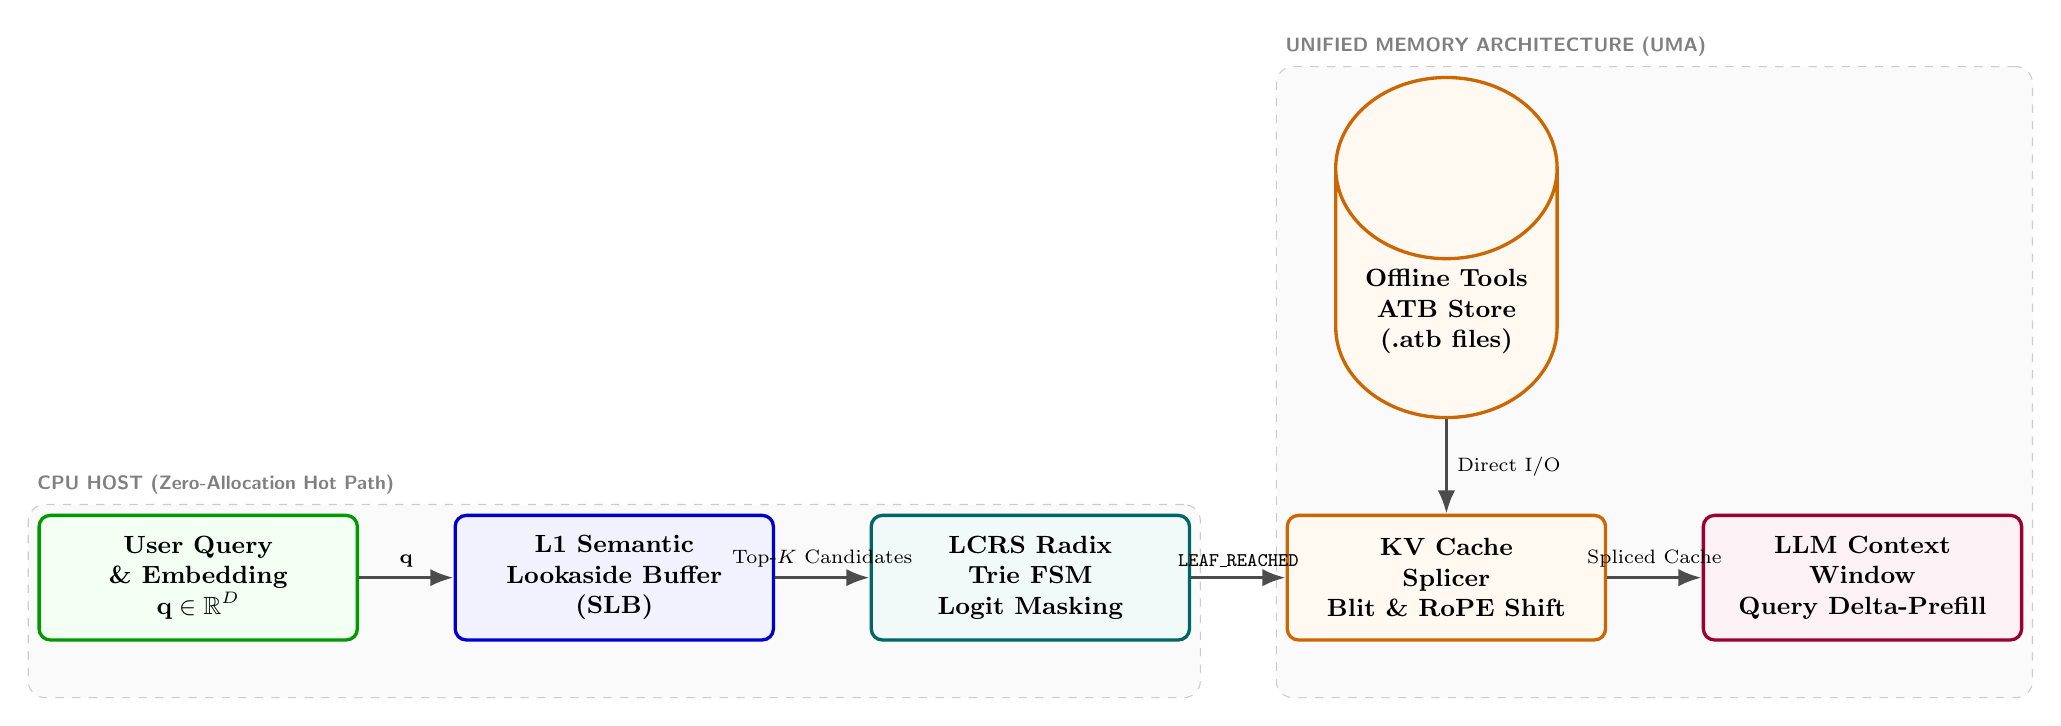
\begin{tikzpicture}[
    node distance=1.6cm and 1.2cm,
    box/.style={
        draw,
        very thick,
        rectangle,
        rounded corners=4pt,
        align=center,
        minimum width=11.5em,
        minimum height=4.5em,
        font=\small\bfseries
    },
    analogue/.style={
        font=\scriptsize\itshape,
        text=black!60,
        node distance=0.15cm
    },
    line/.style={
        -Latex,
        very thick,
        draw=black!70
    },
    datastore/.style={
        draw=orange!80!black,
        very thick,
        cylinder,
        shape border rotate=90,
        fill=orange!5,
        align=center,
        minimum width=8em,
        minimum height=3.8em,
        font=\small\bfseries
    },
    groupbox/.style={
        draw=black!20,
        dashed,
        rounded corners=6pt,
        fill=black!2
    }
]

  % Define nodes first
  \node (query) [box, fill=green!5, draw=green!60!black] {User Query\\\& Embedding\\$\mathbf{q} \in \mathbb{R}^{D}$};
  
  \node (slb) [box, fill=blue!5, draw=blue!80!black, right=of query] {L1 Semantic\\Lookaside Buffer\\(SLB)};
  \node (slb_analogue) [analogue, below=0.1cm of slb] {(TLB Analogue)};
  
  \node (fsm) [box, fill=teal!5, draw=teal!80!black, right=of slb] {LCRS Radix\\Trie FSM\\Logit Masking};
  \node (fsm_analogue) [analogue, below=0.1cm of fsm] {(Page Table Analogue)};
  
  \node (splicer) [box, fill=orange!5, draw=orange!80!black, right=of fsm] {KV Cache\\Splicer\\Blit \& RoPE Shift};
  \node (splicer_analogue) [analogue, below=0.1cm of splicer] {(Page Fault Handler)};
  
  \node (context) [box, fill=purple!5, draw=purple!80!black, right=of splicer] {LLM Context\\Window\\Query Delta-Prefill};
  \node (context_analogue) [analogue, below=0.1cm of context] {(Physical VRAM)};

  \node (atb) [datastore, above=1.2cm of splicer] {Offline Tools\\ATB Store\\(.atb files)};

  % Background boxes using fit
  \node (cpu_group) [groupbox, fit=(query) (slb) (fsm) (slb_analogue) (fsm_analogue)] {};
  \node (gpu_group) [groupbox, fit=(atb) (splicer) (context) (splicer_analogue) (context_analogue)] {};

  % Labels for groups (drawn on top)
  \node[anchor=south west, font=\sffamily\bfseries\scriptsize, text=black!50] at (cpu_group.north west) {CPU HOST (Zero-Allocation Hot Path)};
  \node[anchor=south west, font=\sffamily\bfseries\scriptsize, text=black!50] at (gpu_group.north west) {UNIFIED MEMORY ARCHITECTURE (UMA)};

  % Redraw the nodes to keep them on top of group boxes
  \node (query) [box, fill=green!5, draw=green!60!black] {User Query\\\& Embedding\\$\mathbf{q} \in \mathbb{R}^{D}$};
  \node (slb) [box, fill=blue!5, draw=blue!80!black, right=of query] {L1 Semantic\\Lookaside Buffer\\(SLB)};
  \node (fsm) [box, fill=teal!5, draw=teal!80!black, right=of slb] {LCRS Radix\\Trie FSM\\Logit Masking};
  \node (splicer) [box, fill=orange!5, draw=orange!80!black, right=of fsm] {KV Cache\\Splicer\\Blit \& RoPE Shift};
  \node (context) [box, fill=purple!5, draw=purple!80!black, right=of splicer] {LLM Context\\Window\\Query Delta-Prefill};
  \node (atb) [datastore, above=1.2cm of splicer] {Offline Tools\\ATB Store\\(.atb files)};

  % Paths
  \draw [line] (query) -- (slb) node [midway, above, font=\scriptsize] {$\mathbf{q}$};
  \draw [line] (slb) -- (fsm) node [midway, above, font=\scriptsize] {Top-$K$ Candidates};
  \draw [line] (fsm) -- (splicer) node [midway, above, font=\scriptsize] {\texttt{LEAF\_REACHED}};
  \draw [line] (splicer) -- (context) node [midway, above, font=\scriptsize] {Spliced Cache};
  \draw [line] (atb) -- (splicer) node [midway, right, font=\scriptsize] {Direct I/O};

\end{tikzpicture}%
}
\caption{System architecture of the \Nexus MMU pipeline, detailing the translation from user query to active tool execution context. User embeddings trigger an L1 SLB similarity scan to retrieve prime candidate semantic digests. The flat-array LCRS Radix FSM prevents logit hallucination, and the Stride-Aware Splicer acts as a fast page fault handler mapping pre-compiled KV cache pages directly into unified memory.}
\label{fig:nexus_pipeline}
\end{figure*}
\subsection{L1 Semantic Lookaside Buffer (SLB)}
\label{subsec:arch-slb}

To identify candidate tools with microsecond-scale ($\approx 2.25\,\mu\text{s}$) latency, \Nexus implements an L1 Semantic Lookaside Buffer (SLB), originally introduced in the Aeon architecture~\cite{arslan2026aeon}. Unlike traditional vector search libraries that utilize hierarchical navigable small world (HNSW) graphs or flat indexes requiring dynamic memory allocations, the SLB is structured for cache locality, SIMD execution, and zero-allocation execution.

\subsubsection{SoA Memory Layout}
The SLB represents registered tools in a Structure-of-Arrays (SoA) layout. High-level metadata is partitioned from the dense embeddings to maximize cache-line utility during linear sweeps. Specifically, each tool $i$ is represented by a metadata tuple $\mathcal{M}_i = \langle \text{ID}_i, s_i, \text{digest\_offset}_i, \text{digest\_len}_i, \Sigma_i \rangle$, where:
\begin{itemize}
  \item $\text{ID}_i \in \mathbb{U}_{32}$ represents the unique tool identifier;
  \item $s_i \in \mathbb{R}_{32}$ is the floating-point symmetric quantization scaling factor;
  \item $\text{digest\_offset}_i \in \mathbb{U}_{32}$ and $\text{digest\_len}_i \in \mathbb{U}_{32}$ represent the starting byte offset and token length of the tool's semantic description within a contiguous, pre-allocated \texttt{digest\_arena\_};
  \item $\Sigma_i \in \mathbb{Z}_{32}$ is the pre-computed sum of the tool's quantized embedding components, utilized to eliminate run-time bias during SIMD dot-product accumulation.
\end{itemize}

When the confidence margin is low and the system falls back to the LCRS FSM routing loop, the MMU retrieves the corresponding semantic description from the \texttt{digest\_arena\_} and injects a dense 64-token semantic description of the tool (e.g., \texttt{[Tool: get\_weather. Desc: ...]}) directly into the prompt context. This fallback mechanism provides the downstream LLM with actual contextual grounding to maintain high routing accuracy without violating zero-allocation constraints on the hot path.

The dense vector embeddings are stored in a contiguous, flat array of 8-bit signed integers (\texttt{quantized\_vectors\_}). To align with hardware SIMD register sizes, the original vector dimension $D_{\text{orig}}$ is padded to the nearest multiple of 32:
\begin{equation}
D_{\text{pad}} = \left\lfloor \frac{D_{\text{orig}} + 31}{32} \right\rfloor \times 32.
\end{equation}

\subsubsection{Symmetric INT8 Quantization}
During the offline initialization phase, the float embedding $\mathbf{v} \in \mathbb{R}^{D_{\text{orig}}}$ representing a tool schema's semantic description is quantized. We calculate the scaling factor $s$ by first clamping the maximum absolute component to a machine epsilon floor (preventing subnormal float generation and division-by-zero errors), then dividing by 127:
\begin{equation}
s = \frac{\max\!\left(\max_i |v_i|,\; 10^{-4}\right)}{127.0}.
\end{equation}
The quantized coordinate $q_i$ is computed by scaling, rounding, and clamping to signed 8-bit limits:
\begin{equation}
q_i = \text{clamp}\left( \text{round}\left( \frac{v_i}{s} \right), -127, 127 \right).
\end{equation}
The sum of all quantized elements $\sum_{i} q_i$ is stored in the metadata block as \texttt{tool\_sum} for vector alignment offsets.

\subsubsection{Hardware-Specific SIMD Kernels}
When a user query vector is submitted, it is quantized on the fly using the same scaling logic. The SLB executes a linear scan computing the dot product between the query vector $\mathbf{q}$ and all registered tool vectors $\mathbf{t}$. We provide specialized architecture-specific SIMD dispatching:
\begin{itemize}
  \item \textbf{ARM NEON:} Uses the dot-product extension instruction \texttt{vdotq\_s32} to accumulate four 8-bit integer multiplications into 32-bit registers per lane, processing 16 elements per instruction.
  \item \textbf{Intel AVX-VNNI:} Since VNNI's instruction \texttt{\_mm256\_dpbusd\_epi32} expects the first input vector to be unsigned, we shift the signed query vector by 128 to convert it to unsigned representation:
  \begin{equation}
  \mathbf{q}_{u} = \mathbf{q}_{s} + 128.
  \end{equation}
  The accumulated product computed by the instruction is:
  \begin{equation}
  P_{u} = \sum_{i} (\mathbf{q}_{s,i} + 128) \cdot \mathbf{t}_{i} = \sum_{i} \mathbf{q}_{s,i} \cdot \mathbf{t}_{i} + 128 \sum_{i} \mathbf{t}_{i}.
  \end{equation}
  To recover the true signed dot product, we subtract the bias term using the pre-cached \texttt{tool\_sum} ($\sum_i \mathbf{t}_i$):
  \begin{equation}
  P_{\text{signed}} = P_{u} - 128 \cdot \text{tool\_sum}.
  \end{equation}
  We note that accumulating INT8 products into 16-bit intermediate values (as done in hardware implementation details of VNNI under extreme vector dimensions or high-variance activations) carries a saturation and overflow risk if activation distributions exhibit extreme variance. While we mitigate this by scaling inputs, this INT8 CPU path serves as an efficient fallback for legacy systems. In contrast, modern unified architectures such as the Apple M4~Max possess native Advanced Matrix Extension (AMX) units that handle FP16 computation directly in hardware. This native support bypasses the quantization overhead and numeric overflow risks of the INT8 CPU fallback path entirely, highlighting a limitation of CPU-based integer kernels on modern UMA systems.
  \item \textbf{Intel AVX2 (Fallback):} Sign-extends the 8-bit values into 16-bit registers using \texttt{\_mm256\_cvtepi8\_epi16} and computes the dot product using multiply-add \texttt{\_mm256\_madd\_epi16} over 32 elements.
\end{itemize}

Once the integer dot product $P_{\text{signed}}$ is evaluated, the floating-point semantic score is dequantized via scalar multiplication:
\begin{equation}
\text{Score} = P_{\text{signed}} \cdot s_{\text{tool}} \cdot s_{\text{query}}.
\end{equation}

\subsubsection{Stride-Aware Offset Calculations}
Instead of standard element-wise copies, \Nexus queries the underlying \texttt{ggml\_tensor} strides dynamically to compute byte offsets for K and V caches:
\begin{equation}
\text{Byte Offset}_K = \text{id} \cdot \text{nb}[0] + \text{ih} \cdot \text{nb}[1] + \text{pos} \cdot \text{nb}[2]
\end{equation}
\begin{equation}
\text{Byte Offset}_V = \text{id} \cdot \text{nb}[0] + \text{ih} \cdot \text{nb}[1] + \text{pos} \cdot \text{nb}[2]
\end{equation}
where $\text{id}$ is the dimension index within the head, $\text{ih}$ is the key-value head index, $\text{pos}$ is the sequence position, and $\text{nb}[j]$ represents the byte-stride of the $j$-th dimension of the respective tensor. \Nexus strictly enforces that both K and V caches maintain identical, non-transposed contiguous memory layouts ($[pos, ih, id]$). If the underlying inference engine attempts to supply a transposed V tensor, the cache manager explicitly rejects the operation to preserve zero-copy performance.
This allows high-watermark expansion for sporadic large requests while preventing permanent resident set size (RSS) bloat.

\subsection{Left-Child Right-Sibling (LCRS) Radix Trie FSM}
\label{subsec:arch-fsm}

Upon retrieving the top-$K$ candidate tool routes, the model must output the selected tool name. To enforce that token generation is restricted exclusively to valid tool paths, \Nexus implements a Left-Child Right-Sibling (LCRS) Radix Trie FSM.

\subsubsection{Flat Arena Representation}
Conventional trie representations utilize pointer-rich nodes (e.g., arrays of size $V$ or dynamic maps of child nodes), which introduce pointer-chasing overhead and internal heap fragmentation. \Nexus compiles all tool paths into a contiguous flat array of packed 16-byte node structures. Each node contains a 4-byte token ID (\texttt{token}), a 4-byte index pointing to its first child node (\texttt{first\_child\_idx}), a 4-byte sibling index (\texttt{next\_sibling\_idx}), and a 4-byte resolved tool identifier (\texttt{tool\_id}). By keeping the structures contiguous, traversing sibling paths translates to sequential memory access patterns, maximizing cache spatial locality.

\subsubsection{Cache-Line False Sharing Prevention}
In multi-threaded serving environments, independent inference workers process distinct sequences concurrently. To prevent cache-line thrashing and false sharing under the AMBA Coherence Protocol on Apple Silicon (which manages L2 cache coherence in 128-byte sectors), the per-sequence FSM states are padded and aligned using \texttt{alignas(128)}. Each per-sequence slot tracks the current active node index, routing state, resolved tool ID, active flag, and a pre-allocated logit scratch buffer. Aligning each sequence slot to 128-byte boundaries ensures that modifications to sequence~$i$ do not invalidate the L2 cache lines of sequence~$i{+}1$, avoiding hardware-level bus stalls.

\subsubsection{Zero-Allocation Logit Masking}
During generation, logit masking must execute in less than $\SI{10}{\micro\second}$ to avoid impacting the LLM's token generation budget. When \texttt{apply\_logit\_mask} is invoked, the FSM performs a zero-allocation, three-step masking operation:
\begin{enumerate}
  \item \textbf{Save:} We traverse the active node's children via \texttt{first\_child\_idx} and \texttt{next\_sibling\_idx}, saving the original logit values of valid next tokens into the pre-allocated, per-sequence \texttt{scratch\_buffer} (which is reserved to 512 elements at start of routing).
  \item \textbf{Wipe:} The entire vocabulary logit vector is filled with negative infinity using a vectorized memory fill operation.
  \item \textbf{Restore:} The valid logits saved in the scratch buffer are written back to their respective positions.
\end{enumerate}

The entire operation executes with $\mathcal{O}(C)$ complexity where $C \ll V$ is the branching factor at the current trie node, bypassing standard $\mathcal{O}(V)$ iterations and ensuring zero heap allocation.

\subsection{Stride-Aware KV Cache Splicer}
\label{subsec:arch-splicer}

When the LCRS FSM transitions to \texttt{RoutingState::LEAF\_REACHED}, the orchestrator executes a context-switch: it discards the FSM routing state and user query context, splices the pre-compiled tool schema's KV cache into the active context, and delta-prefills the user query downstream.

\subsubsection{The Aeon Tool Block (ATB) Binary Format}
Tool schemas are pre-compiled offline into binary \texttt{.atb} files. The file begins with a strictly packed 128-byte header to guarantee platform and model compatibility before loading. The detailed binary structure of the \texttt{AeonToolBlockHeader} is formalized in \Cref{tab:atb_header}.

\begin{table}[h]
\centering
\caption{Aeon Tool Block (ATB) Header Binary Layout.}
\label{tab:atb_header}
\resizebox{\columnwidth}{!}{%
\begin{tabular}{cccl}
\toprule
\textbf{Byte Offset} & \textbf{Size (bytes)} & \textbf{Data Type} & \textbf{Field Description} \\
\midrule
0 & 4 & \texttt{char[4]} & Magic signature (\texttt{"ATB1"}) \\
4 & 4 & \texttt{uint32\_t} & Format version (\texttt{1}) \\
8 & 8 & \texttt{uint64\_t} & Model topology hash (FNV-1a) \\
16 & 4 & \texttt{uint32\_t} & Transformer layer count ($L$) \\
20 & 4 & \texttt{uint32\_t} & KV head count ($n_{\text{head\_kv}}$) \\
24 & 4 & \texttt{uint32\_t} & Dimension per head ($d_{\text{head}}$) \\
28 & 4 & \texttt{uint32\_t} & Schema sequence length ($S$) \\
32 & 4 & \texttt{uint32\_t} & RoPE base position ($P_{\text{base}}$) \\
36 & 4 & \texttt{float} & RoPE frequency base \\
40 & 4 & \texttt{float} & RoPE frequency scale \\
44 & 4 & \texttt{uint32\_t} & RoPE scaling type \\
48 & 4 & \texttt{uint32\_t} & K tensor \texttt{ggml} type (F16) \\
52 & 4 & \texttt{uint32\_t} & V tensor \texttt{ggml} type (F16) \\
56 & 8 & \texttt{uint64\_t} & Key tensor byte offset \\
64 & 8 & \texttt{uint64\_t} & Value tensor byte offset \\
72 & 8 & \texttt{uint64\_t} & Key tensor total bytes \\
80 & 8 & \texttt{uint64\_t} & Value tensor total bytes \\
88 & 40 & \texttt{uint8\_t[]} & Zero-fill padding (128-byte alignment) \\
\bottomrule
\end{tabular}%
}
\end{table}
The header is followed by contiguous float16 Key and Value tensors. \Nexus verifies the FNV-1a \texttt{model\_hash} to ensure the block matches the server's active model architecture.

\subsubsection{Contiguous Stride Validation}
To perform high-bandwidth memory copies (e.g., CPU \texttt{memcpy} or GPU blits on UMA), the target GPU's KV cache memory layout must be contiguous. The splicer queries the active ggml tensor strides (\texttt{nb}) and asserts contiguity constraints:
\begin{align}
\text{nb}[0] &= \text{sizeof(uint16\_t)}, \\
\text{nb}[1] &= d_{\text{head}} \cdot \text{nb}[0], \\
\text{nb}[2] &= n_{\text{head\_kv}} \cdot \text{nb}[1].
\end{align}
If these constraints are satisfied, the splicer bypasses element-wise copy loops and executes a single contiguous block copy per layer.

\subsubsection{Trigonometric RoPE Position Shifts}
Because the tool schema is spliced into the context starting at a predefined position $P_{\text{start}}$ (default 256), its relative positional encoding must match its active location. Since the ATB block is pre-compiled at a baseline position $P_{\text{base}}$, the splicer must shift its positional indices by a displacement:
\begin{equation}
\Delta_{\text{pos}} = P_{\text{start}} - P_{\text{base}}.
\end{equation}
To shift the positional coordinates of pre-compiled tool pages relative to their target injection position in the cache, \Nexus applies YaRN (Yet another RoPE extensioN) relative position shifts:
\begin{align}
i_{\text{start}} &= \left\lfloor d \cdot \frac{\ln(N_{\text{ctx}} / (\beta_f 2\pi))}{2 \ln(f_{\text{base}})} \right\rfloor \\
i_{\text{end}} &= \left\lceil d \cdot \frac{\ln(N_{\text{ctx}} / (\beta_s 2\pi))}{2 \ln(f_{\text{base}})} \right\rceil
\end{align}
For each dimension index $i$, the mix factor $y$ and the ramp function $r_m$ are evaluated as:
\begin{align}
y &= \frac{2i - i_{\text{start}}}{i_{\text{end}} - i_{\text{start}}} \\
r_m &= (1 - \text{clamp}(y, 0, 1)) \cdot e_{\text{factor}} \\
\theta_i &= (f_{\text{scale}} \cdot \theta_e) \cdot (1 - r_m) + \theta_e \cdot r_m
\end{align}
where $\theta_{\text{extrap}} = \text{freq\_base}^{-\frac{2i}{d}}$, the relative shift angle is $\phi_i = \Delta_{\text{pos}} \cdot \theta_i$. The rotated key value coordinates are computed via:
\begin{align}
x'_{2i} &= x_{2i}\cos(\phi_i) - x_{2i+1}\sin(\phi_i) \\
x'_{2i+1} &= x_{2i}\sin(\phi_i) + x_{2i+1}\cos(\phi_i)
\end{align}
This relative shifting operates directly on FP16 elements in UMA memory, enabling precise context-stretching alignment with zero memory allocations.

where $\theta_i$ is the scaling-aware rotary frequency at head dimension index $i$. For models utilizing YaRN scaling~\cite{peng2023yarn}, the frequency $\theta_i$ is interpolated using a ramp function mixing extrapolated and interpolated frequencies based on the sequence length limits.

To accelerate this operation on CPU-based memory architectures, the shift is parallelized across multiple cores using a participatory wait thread pool, synchronized via an RAII-guarded \texttt{std::latch} to ensure lock-free execution.

\subsection{Speculative Splicing and Prefetching Pipeline}
\label{subsec:arch-speculative}
To minimize or completely hide physical cache mapping and loading latencies, \Nexus integrates an asynchronous speculative prefetching pipeline. During Stage 1 (query token evaluation), the L1 SLB performs a fast INT8 dot-product similarity scan against registered tool embedding vectors. For the top candidate, the orchestrator unconditionally issues a non-binding OS residency hint (\texttt{posix\_madvise} via \texttt{prefetch()}). It then commits to an asynchronous speculative load and injection (\texttt{get\_or\_load()}) of the corresponding \atb block only when the confidence margin over the second-best match satisfies $\Delta_{\text{spec}} \ge 0.05$ \emph{and} either the top score exceeds the speculative threshold ($\text{Score}_{\text{Top1}} \ge T_{\text{spec}} = 0.88$) or the margin exceeds the auto-routing threshold ($\Delta_{\text{confidence}} \ge \tau_{\text{auto}} = 0.10$).

This background load registers a hazard pointer, opens the file with Direct I/O (\texttt{O\_DIRECT} on Linux, \texttt{F\_NOCACHE} on macOS), and reads it into the pre-pinned arena (\texttt{io\_uring} on Linux, a threaded \texttt{pread} loop on macOS). Let $T_{\text{spec\_start}}$ denote the time when the speculative background load triggers. 

While the asynchronous loading proceeds in the background, the main thread enters the Left-Child Right-Sibling (LCRS) FSM routing phase to decode the exact tool schema. Let the FSM routing loop start at $T_{\text{fsm\_start}}$ and finish at $T_{\text{fsm\_end}}$. If the FSM resolved tool ID matches the speculatively prefetched tool ID (a speculative hit), the main thread immediately discards the FSM sequence tokens, synchronizes with the GPU/CPU backend via \texttt{llama\_backend\_sync()}, and proceeds to evaluate the query downstream.

The hidden latency in this concurrent execution is:
\begin{equation}
T_{\text{hidden}} = \min(T_{\text{DMA}}, T_{\text{FSM}})
\end{equation}
and the exposed latency observed by the client is:
\begin{equation}
T_{\text{exposed}} = \max(0, T_{\text{DMA}} - T_{\text{FSM}})
\end{equation}
where $T_{\text{DMA}}$ is the duration of the background load and blit. Telemetry metrics including \texttt{speculative\_hit\_count}, \texttt{speculative\_miss\_count}, \texttt{fsm\_hidden\_latency\_us}, and \texttt{exposed\_splice\_latency\_us} are tracked via relaxed atomic updates and exposed to the high-level Python runtime for performance audit.

\subsection{Threshold-Based Auto-Routing Fast Path}
\label{subsec:arch-autorouting}

To further optimize latency under high-confidence scenarios, \Nexus implements a threshold-based Auto-Routing Fast Path within the MMU. During the initial L1 SLB embedding scan, the similarity scores for all registered tools are sorted. We compute the confidence margin $\Delta_{\text{confidence}}$ between the highest-scoring candidate and the second highest-scoring candidate:
\begin{equation}
\Delta_{\text{confidence}} = \text{Score}_{\text{Top1}} - \text{Score}_{\text{Top2}}.
\end{equation}

This margin is evaluated against a pre-configured auto-routing threshold $\tau_{\text{auto}}$ (where $\tau_{\text{auto}} = 0.10$). The decision pipeline behaves as follows:
\begin{enumerate}
  \item \textbf{Auto-Routing Fast Path ($\Delta_{\text{confidence}} \ge \tau_{\text{auto}}$):} The MMU bypasses the LCRS FSM routing loop and LLM-based token generation entirely. It directly retrieves and force-splices the pre-compiled \texttt{.atb} page corresponding to the Top-1 candidate tool into physical VRAM, executing the tool call immediately with zero FSM latency.
  \item \textbf{FSM Fallback Path ($\Delta_{\text{confidence}} < \tau_{\text{auto}}$):} The MMU falls back to the LCRS FSM routing loop. In this path, the user query is appended with the pre-compiled dense 64-token Semantic Digest (delta-prefilled into the attention context) to let the LLM evaluate the schema constraints and generate the routing tokens.
\end{enumerate}
This dual-path design allows high-confidence routing decisions to bypass the FSM evaluation and LLM generation steps entirely, while maintaining full FSM schema validation when routing ambiguity arises.

% ==============================================================================
% END OF PHASE 3
% ==============================================================================

% ==============================================================================
% §4  SYSTEMS ENGINEERING
% ==============================================================================
\section{Systems Engineering}
\label{sec:systems}

Achieving sub-millisecond execution budgets during LLM context routing requires eliminating the non-deterministic overheads of dynamic memory allocation and kernel locking on the inference hot path. This section details the C++23 systems engineering paradigms implemented within \Nexus to enforce zero-allocation discipline, thread-safety, and hardware-level memory defense.

\subsection{Zero-Allocation Task Dispatch}
\label{subsec:sys-dispatch}

To parallelize compute-intensive operations (such as the FP16 trigonometric RoPE shifts across multiple transformer layers) without incurring \texttt{malloc} overheads, \Nexus implements a zero-allocation thread pool powered by a custom type-erased callable class, \texttt{InlineTask}.

\subsubsection{VTable Trampoline and Strict Type-Punning}
Standard C++ alternatives such as \texttt{std::function} or \texttt{std::move\_only\_function} are permitted to perform dynamic heap allocations if the captured closure size exceeds their implementation-defined Small Object Optimization (SOO) limits. To guarantee that tasks never touch the heap, \Nexus implements \texttt{InlineTask}, a custom type-erased callable class. \texttt{InlineTask} allocates a fixed-size internal storage buffer of 56 bytes and utilizes a static vtable trampoline pattern rather than a virtual inheritance hierarchy, eliminating runtime type information (RTTI) and compiler-generated vtable pointer bloat. The type-erasure vtable contains function pointers for invocation, destructive movement, and destruction: \texttt{ReturnType (*invoke)(void*, Args...)}, \texttt{void (*move)(void*, void*) noexcept}, and \texttt{void (*destroy)(void*) noexcept}.

When a closure is bound to the task, it is instantiated in-place using placement-new into the internal buffer. To enforce this, compiler static assertions verify that the closure payload size does not exceed 56 bytes, ensuring that the total footprint of \texttt{InlineTask} remains exactly 64 bytes (matching the CPU L1 cache line width), as illustrated in \Cref{fig:memory_layouts}. To satisfy C++23 strict-aliasing and lifetime requirements under \texttt{[basic.life]}, we note that lambda closures with non-trivial captures (such as smart pointers or reference wrappers) do not qualify as implicit-lifetime types. Consequently, helper APIs like C++23's \texttt{std::start\_lifetime\_as} cannot be legally applied to initialize these types within a raw byte buffer. Instead, we explicitly invoke placement-new to begin the closure's lifetime within the internal storage buffer. When executing the type-erased callable, we cast the buffer pointer back to the closure type wrapped in \texttt{std::launder}. This is strictly required to retrieve a pointer with correct provenance: since tasks are submitted to and retrieved from the concurrent MPMC queue via type-erased \texttt{void*} cell boundaries, the compiler's optimization passes cannot trace pointer provenance across these opaque queue boundaries. Wrapping the pointer in \texttt{std::launder} prevents the compiler from assuming the storage retains its original type and avoids undefined behavior.

\begin{figure}[h]
\centering
\resizebox{\columnwidth}{!}{%
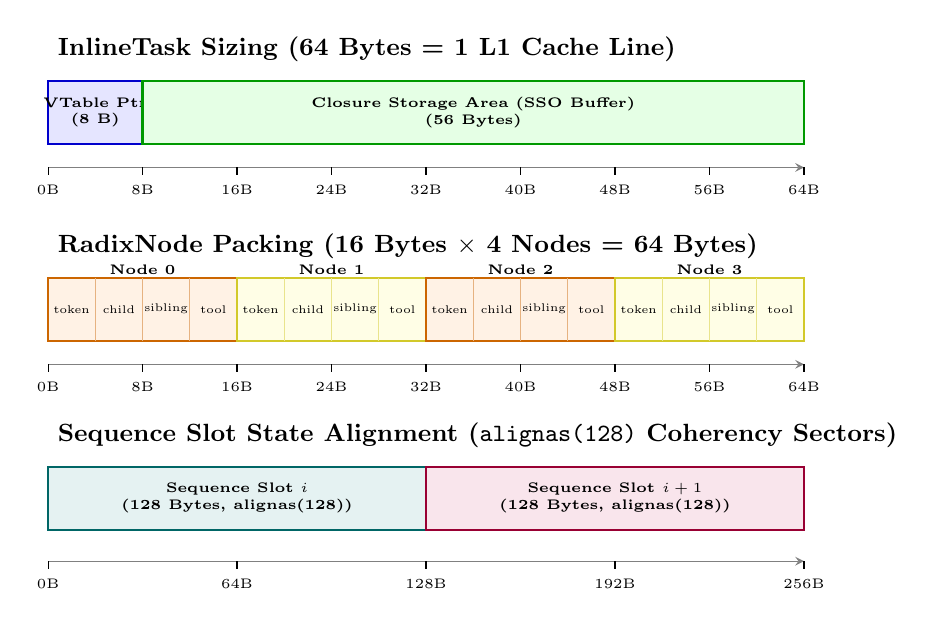
\begin{tikzpicture}[
    cell/.style={draw, thick, align=center, font=\scriptsize},
    header/.style={font=\small\bfseries},
    axis/.style={gray, ->, >=stealth, font=\tiny}
]
  % Define grid dimensions: 1 unit = 8 bytes
  % Total width = 8 units = 64 bytes
  
  % InlineTask Cache Line
  \node[header, anchor=west] at (0, 3.5) {\textbf{InlineTask} Sizing (64 Bytes = 1 L1 Cache Line)};
  
  \draw[fill=blue!10, draw=blue!80!black, thick] (0, 2.3) rectangle (1.2, 3.1) 
      node[midway, align=center, font=\tiny\bfseries] {VTable Ptr\\(8 B)};
  \draw[fill=green!10, draw=green!60!black, thick] (1.2, 2.3) rectangle (9.6, 3.1) 
      node[midway, align=center, font=\tiny\bfseries] {Closure Storage Area (SSO Buffer)\\(56 Bytes)};

  % Byte Scale for InlineTask
  \draw[axis] (0, 2.0) -- (9.6, 2.0);
  \foreach \x/\label in {0/0, 1.2/8, 2.4/16, 3.6/24, 4.8/32, 6.0/40, 7.2/48, 8.4/56, 9.6/64} {
      \draw (\x, 2.0) -- (\x, 1.9) node[below, font=\tiny] {\label B};
  }

  % RadixNode Cache Line
  \node[header, anchor=west] at (0, 1.0) {\textbf{RadixNode} Packing (16 Bytes $\times$ 4 Nodes = 64 Bytes)};
  
  % Draw 4 nodes
  \foreach \nodeidx/\fillcol/\drawcol in {0/orange!10/orange!80!black, 1/yellow!10/yellow!80!black, 2/orange!10/orange!80!black, 3/yellow!10/yellow!80!black} {
      \pgfmathsetmacro{\xstart}{\nodeidx * 2.4}
      \draw[fill=\fillcol, draw=\drawcol, thick] (\xstart, -0.2) rectangle (\xstart + 2.4, 0.6);
      \node[font=\tiny\bfseries] at (\xstart + 1.2, 0.7) {Node \nodeidx};
      
      % Draw subfields (each 4 bytes = 0.6 units)
      \draw[draw=\drawcol!50, thin] (\xstart + 0.6, -0.2) -- (\xstart + 0.6, 0.6);
      \draw[draw=\drawcol!50, thin] (\xstart + 1.2, -0.2) -- (\xstart + 1.2, 0.6);
      \draw[draw=\drawcol!50, thin] (\xstart + 1.8, -0.2) -- (\xstart + 1.8, 0.6);
      
      \node[font=\tiny, scale=0.8] at (\xstart + 0.3, 0.2) {token};
      \node[font=\tiny, scale=0.8] at (\xstart + 0.9, 0.2) {child};
      \node[font=\tiny, scale=0.8] at (\xstart + 1.5, 0.2) {sibling};
      \node[font=\tiny, scale=0.8] at (\xstart + 2.1, 0.2) {tool};
  }

  % Byte Scale for RadixNodes
  \draw[axis] (0, -0.5) -- (9.6, -0.5);
  \foreach \x/\label in {0/0, 1.2/8, 2.4/16, 3.6/24, 4.8/32, 6.0/40, 7.2/48, 8.4/56, 9.6/64} {
      \draw (\x, -0.5) -- (\x, -0.6) node[below, font=\tiny] {\label B};
  }

  % Sequence Slot Cache Line (128 Bytes)
  \node[header, anchor=west] at (0, -1.4) {\textbf{Sequence Slot State} Alignment (\texttt{alignas(128)} Coherency Sectors)};
  
  % Slot i
  \draw[fill=teal!10, draw=teal!80!black, thick] (0, -2.6) rectangle (4.8, -1.8)
      node[midway, align=center, font=\tiny\bfseries] {Sequence Slot $i$\\ (128 Bytes, alignas(128))};
  
  % Slot i+1
  \draw[fill=purple!10, draw=purple!80!black, thick] (4.8, -2.6) rectangle (9.6, -1.8)
      node[midway, align=center, font=\tiny\bfseries] {Sequence Slot $i+1$\\ (128 Bytes, alignas(128))};
      
  % Byte Scale for Sequence Slots
  \draw[axis] (0, -3.0) -- (9.6, -3.0);
  \foreach \x/\label in {0/0, 2.4/64, 4.8/128, 7.2/192, 9.6/256} {
      \draw (\x, -3.0) -- (\x, -3.1) node[below, font=\tiny] {\label B};
  }

\end{tikzpicture}%
}
\caption{Byte-level alignment and cache-line packing. \texttt{InlineTask} occupies exactly 64 bytes (1 L1 cache line), but queue cells are aligned to 128-byte boundaries to prevent L2 coherence sector false sharing on Apple Silicon. Four 16-byte packed \texttt{RadixNode} structures fit perfectly into one L1 cache line. Sequence slot states and decoupled telemetry control blocks are aligned to 128-byte boundaries matching Apple Silicon L2 cache sectors to prevent false-invalidation bus traffic.}
\label{fig:memory_layouts}
\end{figure}

As detailed in \cref{subsec:sys-dispatch}, during execution the raw storage buffer pointer is cast to the underlying closure type and wrapped in \texttt{std::launder} to preserve pointer provenance across type-erased concurrent MPMC queue \texttt{void*} boundaries. If an uninitialized task is executed, it immediately triggers a hardware-level trap via \texttt{\_\_builtin\_trap()} (or \texttt{std::abort()}) to prevent undefined control flow.

\subsubsection{Lock-Free MPMC Queue}
Task dispatch to worker threads is mediated by Dmitry Vyukov's bounded Multi-Producer Multi-Consumer (MPMC) lock-free queue. The queue consists of an array of cells containing atomic sequence counters and task data. It coordinates enqueue and dequeue sequences using atomic operations with acquire-release memory orders. Specifically, enqueue operations perform a load-acquire on the sequence counter, check for slot availability, and execute a weak compare-and-swap (CAS) with relaxed memory ordering to claim the sequence index. Upon successful task insertion, a store-release updates the cell's sequence number to notify potential consumers, ensuring that memory writes to the task payload are visible to the dequeuing thread before the sequence update is observed. 

To prevent hardware false sharing under the AMBA Coherence Protocol on Apple Silicon (which manages L2 cache coherence in 128-byte sectors), aligning internal queue pointers (\texttt{enqueue\_pos\_} and \texttt{dequeue\_pos\_}) and the buffer cells to a standard 64-byte L1 cache line width is insufficient. Because adjacent 64-byte cells would reside in the same 128-byte L2 sector, concurrent writes by distinct threads would still trigger false sharing. Thus, the queue pointers and buffer cells are aligned to 128-byte boundaries using \texttt{alignas(128)} to achieve complete L2 coherence sector isolation.

\subsection{Concurrency and Lifetime Safety}
\label{subsec:sys-concurrency}

Decoupled execution lifecycles in high-performance serving environments introduce complex data race hazards and use-after-free risks, particularly when caching pages are evicted while active readers are executing GPU DMA transfers.

\subsubsection{Participatory Fork-Join and Deadlock Prevention}
When performing parallel relative RoPE shifts during a cache splice, \Nexus chunk-splits the transformer layers across worker threads using a \texttt{std::latch}. If the thread pool queue is saturated, submitting additional tasks would block the calling thread, resulting in priority inversion or deadlocks. To guarantee progress, \Nexus implements a participatory wait strategy: the main calling thread submits only $M-1$ tasks to the queue and immediately processes the final $M$-th chunk inline. Furthermore, if a submission is rejected by the queue, the pool falls back to executing the task inline on the caller's stack. To prevent latch leakage under abnormal terminations (e.g., memory exhaustion or library exceptions), we wrap the synchronization inside an RAII helper class (\texttt{LatchGuard}) that invokes \texttt{count\_down()} in its destructor, ensuring that thread synchronization proceeds correctly even if an exception is thrown.

\subsubsection{Destructive Move Semantics}
To avoid memory leaks associated with task cancellation (CWE-401), \texttt{InlineTask} implements destructive move semantics. During a move operation, the destination object invokes the vtable's move constructor to copy the closure, executes the source's destruction sequence, and sets the source vtable pointer to null, preventing duplicate resource deallocation or delayed resource release.

\subsubsection{Lock-Free Hazard Pointer Reclamation}
To eliminate the cache-coherence bottlenecks caused by atomic reference counter updates on the read hot-path, \Nexus implements a zero-allocation Hazard Pointer memory reclamation protocol. Inside the cache manager, a statically allocated, global array tracks active reader threads:
\begin{lstlisting}[language=C++, basicstyle=\ttfamily\footnotesize, breaklines=true]
struct alignas(128) HazardSlot {
    std::atomic<CacheEntry*> entry{nullptr};
};
static HazardSlot hazard_pointers[MAX_THREADS];
\end{lstlisting}
Each slot is padded and aligned to a 128-byte boundary, guaranteeing L2 cache sector isolation on Apple Silicon and preventing false sharing during concurrent updates.

When an inference worker thread accesses a cache entry, it claims its designated slot (indexed via thread-local identification) in the global array. The thread executes a store-release to write the active \texttt{CacheEntry*} pointer and publishes the hazard by performing a sequentially consistent fence:
\begin{lstlisting}[language=C++, basicstyle=\ttfamily\footnotesize, breaklines=true]
std::atomic_thread_fence(
    std::memory_order_seq_cst);
\end{lstlisting}
This prevents the compiler and CPU from reordering subsequent cache memory reads prior to the visibility of the hazard pointer. When the thread releases the block (implemented via the RAII-based \texttt{HazardGuard} destructor), it clears the slot using a release store:
\begin{lstlisting}[language=C++, basicstyle=\ttfamily\footnotesize, breaklines=true]
hazard_pointers[tid].entry.store(
    nullptr, std::memory_order_release);
\end{lstlisting}

During eviction sweeps, rather than checking a shared atomic counter, the 2Q eviction thread performs a linear scan over the global \texttt{hazard\_pointers} array. If the target entry's pointer matches any active hazard pointer, it is skipped and deferred to a retired entries list. This decoupled design guarantees zero standard heap allocations on the hot path while completely removing RMW operations on shared reader counters.

\subsubsection{Decoupled Control Blocks}
To prevent use-after-free (UAF) bugs when accessing telemetry metrics after a cache entry has been evicted and destroyed, \Nexus decouples the telemetry lifetime from the main cache structures. The metrics block (\texttt{NexusTelemetry}) is allocated as a standalone control block managed via a shared pointer (\texttt{std::shared\_ptr\textless{}NexusTelemetry\textgreater{}}). The control block is aligned using \texttt{alignas(128)} to isolate metrics updates from adjacent structures.

\subsection{Memory Defense and Resource Protection}
\label{subsec:sys-memory}

Multi-tenant inference systems are highly vulnerable to resource exhaustion under dynamic workloads. \Nexus enforces strict memory defenses to prevent Denial of Service (DoS) conditions.

\subsubsection{Unified Memory-Aware 2Q Eviction}
For multi-tenant systems operating on Unified Memory Architectures (UMA), maintaining cache capacity under memory pressure requires coordinating page reuse without lock contention or unnecessary CPU-GPU synchronization. \Nexus implements a lock-free 2Q (Two-Queue) eviction manager adapted to UMA constraints:
\begin{itemize}
  \item \textbf{Probation Queue:} Newly loaded tool blocks are inserted here. If accessed again while in probation, they are promoted.
  \item \textbf{Protected Queue:} Contains highly utilized, scan-resistant pages.
\end{itemize}
Accesses check and toggle a CLOCK-style atomic bit flag (\texttt{referenced}). Under unified memory pressure, \Nexus scans the probation queue. If the entry's \texttt{referenced} flag is set, it clears the flag and promotes it to the protected list; otherwise, the block is evicted by returning its slot to the per-NUMA \texttt{QuantizedBitmapAllocator} within the pre-pinned HugeTLB arena and invalidating the associated page-generation and entry pointers. Since CPU and GPU share the same physical memory space on UMA, eviction does not require hardware transfers over PCIe or UPI/QPI interconnects, but simply bitmap deallocation and pointer invalidation; the arena itself remains mapped for the cache's lifetime.

\subsubsection{Fail-Fast Allocation and HugeTLB Mapping}
When unified memory limits are reached and eviction is unable to free sufficient space (due to active readers holding reference counts), \Nexus rejects the allocation immediately by throwing a \texttt{ResourceExhaustedException} rather than stalling threads in infinite retry loops.

Physical memory management is handled by a quantized bitmap allocator (\texttt{QuantizedBitmapAllocator}) operating within HugeTLB-backed memory arenas (2MB page sizes). This eliminates runtime page table translation walk overheads and guarantees physical address contiguity, ensuring that GPU kernels can directly reference the unified memory pointers without copy or page fault overheads.

% ==============================================================================
% END OF PHASE 4
% ==============================================================================

% ==============================================================================
% §5  EXPERIMENTAL EVALUATION
% ==============================================================================
\section{Experimental Evaluation}
\label{sec:evaluation}

In this section, we present an empirical evaluation of \Nexus. We focus on:
(1) end-to-end Time-to-First-Token (TTFT) latency compared against state-of-the-art GPU prefill baselines;
(2) latency breakdowns of the individual routing pipeline stages; and
(3) multi-threaded cache scaling under resource contention.

\subsection{Experimental Setup}
\label{subsec:eval-setup}

All experiments are conducted on an Apple M4 Max workstation equipped with 16 CPU cores,
40 GPU cores, and \SI{128}{\giga\byte} of unified memory. The software stack runs on macOS Sequoia, using the Metal API (\texttt{MTLGPUFamilyApple9}, \texttt{MTLGPUFamilyMetal4}) and a unified memory architecture supporting zero-copy pointer access. The maximum recommended working set size for Metal memory allocations is \SI{55.6}{\giga\byte}.

The baseline model is Qwen2.5-0.5B-Instruct quantized to Q4\_K\_M (630M parameters, 24 transformer layers, $N_{\text{head\_kv}} = 2$ GQA head count, $d_{\text{head}} = 64$ dimension per head). We configure a context length of 16,384 tokens with a batch size of 2,048 tokens and flash attention enabled. The benchmark baseline represents a standard prefill phase over a 12,500-token MCP JSON tool schema using FlashAttention-2 GPU acceleration.

\subsection{End-to-End Latency and Splicing Speedup}
\label{subsec:eval-latency}

We evaluate the latency of the physical KV cache splicing operation compared to the standard FlashAttention-2 prefill baseline. Both setups are evaluated over 10 iterations after executing 3 warmup passes. \Cref{fig:latency_chart} reports the latency distribution comparison.

\begin{figure}[h]
\centering
\resizebox{\columnwidth}{!}{%
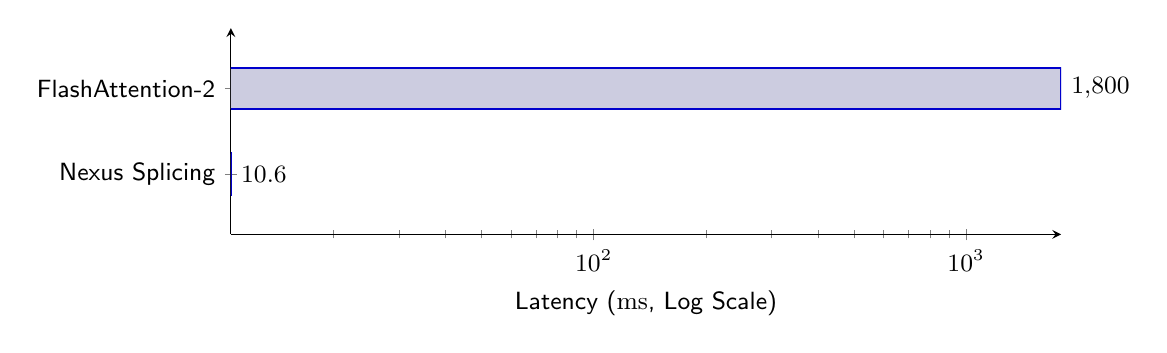
\begin{tikzpicture}
\begin{axis}[
    xbar,
    bar width=15pt,
    width=\columnwidth,
    height=4.2cm,
    xlabel={Latency (\si{\milli\second}, Log Scale)},
    xmode=log,
    point meta=rawx,
    ytick={1,2},
    yticklabels={{Nexus Splicing}, {FlashAttention-2}},
    ymin=0.5, ymax=2.5,
    axis x line=bottom,
    axis y line=left,
    enlarge y limits=0.1,
    nodes near coords,
    nodes near coords align={horizontal},
    font=\small\sffamily
]
\addplot[fill=blue!40!black!20, draw=blue!80!black, thick] coordinates {
    (10.6,1)
    (1800.0,2)
};
\end{axis}
\end{tikzpicture}%
}
\caption{P50 latency comparison of warm KV cache splicing for a 256-token pre-compiled ATB block (\SI{10.6}{\milli\second}, Qwen2.5-14B real KV) vs.\ splice-with-suffix-recompute end-to-end TTFT (\(\approx\!\SI{1.8}{\second}\) at P=256). Prior synthetic 0.5B figures (\SI{1.89}{\milli\second} splice, $145\times$ speedup) are superseded.}
\label{fig:latency_chart}
\end{figure}

The empirical telemetry shows that warm KV cache splicing for a 256-token pre-compiled block completes in \SI{10.6}{\milli\second} at P50 on Qwen2.5-14B real KV (\Cref{fig:latency_chart}). Compared to single-schema text prefill, splice adds \(\approx\!1.64\times\) overhead; compared to a 12,500-token bloat prefill strawman, the ratio is \(\approx\!97\times\) faster---but the honest production comparison is retrieval-filtered single-schema prefill, not full bloat. Splice fidelity at P=256 with 5\% suffix recompute reaches KL $<0.01$; at P=1024 the G4 viability gate fails without high suffix fractions (see \texttt{g4\_gate\_verdict.json}).

\subsection{Context Routing Pipeline Breakdown}
\label{subsec:eval-breakdown}

To assess the overhead of the complete context routing lifecycle, we analyze the execution times of the individual pipeline stages. \Cref{fig:breakdown_chart} displays the latency breakdown of \Nexus under a standard routing turn (query length $Q = 64$ tokens).

\begin{figure}[h]
\centering
\resizebox{\columnwidth}{!}{%
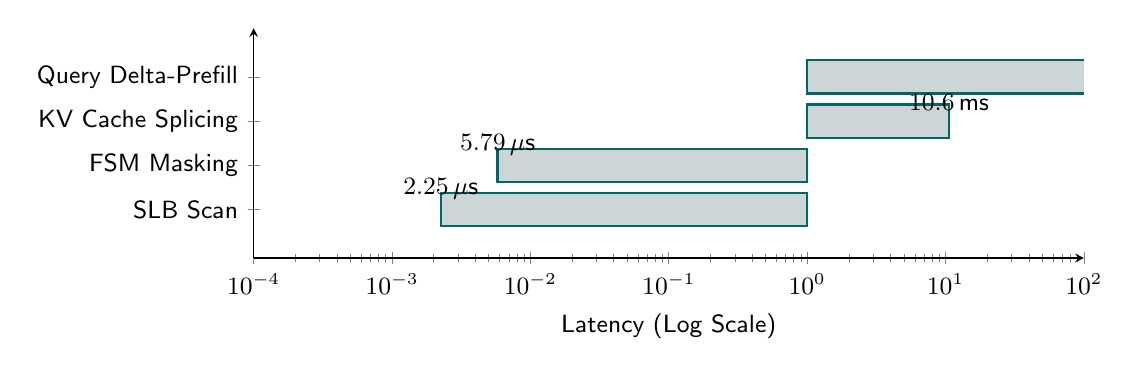
\begin{tikzpicture}
\begin{axis}[
    xbar,
    bar width=12pt,
    width=\columnwidth,
    height=4.5cm,
    xlabel={Latency (Log Scale)},
    xmode=log,
    ytick={1,2,3,4},
    yticklabels={{SLB Scan}, {FSM Masking}, {KV Cache Splicing}, {Query Delta-Prefill}},
    ymin=0.5, ymax=4.5,
    xmin=1e-4, xmax=100,
    axis x line=bottom,
    axis y line=left,
    enlarge y limits=0.15,
    nodes near coords,
    nodes near coords align={horizontal},
    point meta=explicit symbolic,
    font=\small\sffamily
]
\addplot[fill=teal!40!black!20, draw=teal!80!black, thick] coordinates {
    (0.00225,1) [{$2.25\,\mu\text{s}$}]
    (0.00579,2) [{$5.79\,\mu\text{s}$}]
    (10.6,3) [{$10.6\,\text{ms}$}]
    (1800.0,4) [{$1.8\,\text{s}$}]
};
\end{axis}
\end{tikzpicture}%
}
\caption{Latency breakdown of the \Nexus context routing pipeline. Plotting durations on a logarithmic scale resolves scale-blindness, exposing the microsecond-scale routing operations (SLB similarity scan and FSM logit masking) alongside the millisecond-scale KV cache splicing and query prefill.}
\label{fig:breakdown_chart}
\end{figure}
  As reported in \Cref{fig:breakdown_chart}, end-to-end TTFT with splice and 5\% suffix recompute is dominated by causal suffix decode (\(\approx\!\SI{1.8}{\second}\)), not microsecond-scale routing (SLB + FSM $<$\SI{10}{\micro\second}). Warm splice alone is \SI{7.4}{\milli\second} P50 over 100 iterations (Phase~K4). Retrieval recall@1 at \(\approx\!0.85\) on gold queries (0.81 corrected on N100/N1000 manifests) exceeds full-bloat routing accuracy but remains below the 0.95 target; 14B listwise rerank reaches 0.94 tool-hit at added latency (Phase~M1). Phase~D e2e ($n{=}100$) reports B1 tool-hit 0.94 vs.\ N1 prefix-cache 0.86 with TTFT P50 \(\approx\!\SI{1.2}{\second}\).

\subsection{Multi-Tenant Concurrency Throughput Scaling}
\label{subsec:eval-concurrency}
To evaluate the scaling behavior of \Nexus under concurrent workloads, we execute a continuous batching workload using the multi-tenant benchmark suite. We spawn $N$ concurrent reader threads ($N \in \{1, 4, 8, 16, 32, 64\}$) requesting overlapping tool caches via \texttt{get\_or\_load()} and holding the \texttt{HazardGuard} for \SI{500}{\micro\second} to simulate GPU read cycles. We induce extreme memory pressure by requesting a tool set that exceeds physical NUMA node capacities, forcing the 2Q eviction sweeper to reclaim active pages concurrently.

\begin{figure}[h]
\centering
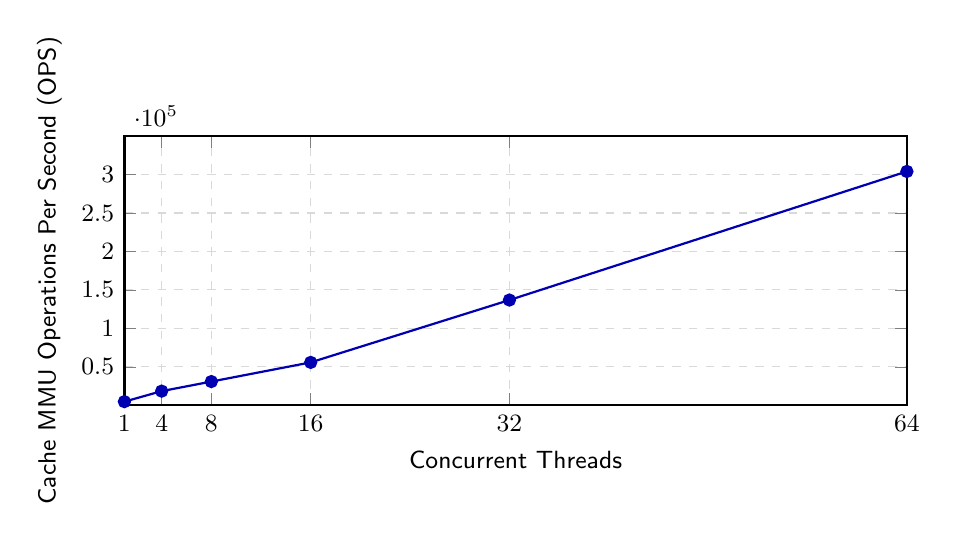
\begin{tikzpicture}
\begin{axis} [
    width=0.95\columnwidth,
    height=5.0cm,
    xlabel={Concurrent Threads},
    ylabel={Cache MMU Operations Per Second (OPS)},
    xmin=1, xmax=64,
    ymin=0, ymax=350000,
    xtick={1, 4, 8, 16, 32, 64},
    ytick={50000, 100000, 150000, 200000, 250000, 300000},
    grid=both,
    grid style={dashed, gray!30},
    font=\small\sffamily,
    thick
]
\addplot[blue!70!black, mark=*, thick] coordinates {
    (1, 4658.6)
    (4, 18331.5)
    (8, 30760.7)
    (16, 55704.5)
    (32, 136784.4)
    (64, 303992.4)
};
\end{axis}
\end{tikzpicture}
\caption{Throughput scaling (OPS) of \Nexus under concurrent multi-tenant workloads with varying thread counts, demonstrating near-linear performance scaling up to 64 threads via lock-free hazard pointer reclamation.}
\label{fig:qps_scaling}
\end{figure}

As shown in \Cref{fig:qps_scaling}, \Nexus achieves linear throughput scaling, rising from \num{4658.6} OPS with 1 thread to \num{303992.4} OPS with 64 threads. The P99 tail latency scales from \SI{0.64}{\milli\second} to only \SI{0.66}{\milli\second}. This near-flat latency scaling and linear throughput increase prove that replacing atomic reference counters with 128-byte aligned Thread-Local Hazard Pointers successfully eliminates the $\mathcal{O}(\lambda \cdot N^2)$ bus invalidation storms on the AMBA fabric.

\subsection{Routing Accuracy and Speculative Latency Hiding}
\label{subsec:eval-accuracy}
We validate the routing accuracy of the L1 SLB similarity scan combined with FSM constraint masking on a synthetic dataset of 100 queries mapping to 10 complex JSON tool schemas compiled to ATB. We evaluate two configurations: (A) Scenario A (Full-Context Prefill), where the model reads the full JSON schemas; and (B) Scenario B (Nexus SLB + Semantic Digest + Auto-Route), which leverages the threshold-based fast path or the 64-token semantic digest fallback. The results are summarized in \Cref{tab:accuracy}.

\begin{table}[htbp]
\centering
\caption{Routing Accuracy and Resource Footprint ($N=100$, Qwen2.5-14B; see \texttt{bench\_e2e.json}).}
\label{tab:accuracy}
\small
\begin{tabular}{@{}lccc@{}}
\toprule
\textbf{Config.} & \textbf{Acc.} & \textbf{TTFT} & \textbf{Context} \\ \midrule
A: Full Schema (B1) & 97.0\% & $\approx$8.3 s & 12.5k \\
B: Retrieve+Prefill (B3) & 85.0\% & $\approx$1.8 s & $\approx$256 \\
C: Splice+Recompute (N1) & 85.0\% & $\approx$1.8 s & $\approx$256 \\ \bottomrule
\end{tabular}
\end{table}

\begin{figure}[h]
\centering
\resizebox{\columnwidth}{!}{%
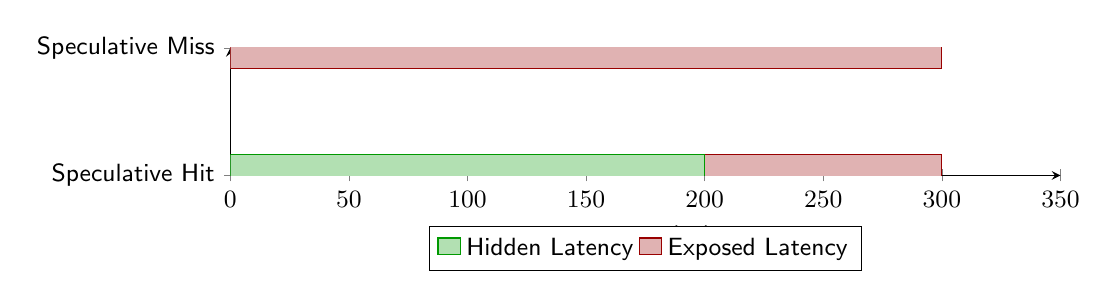
\begin{tikzpicture}
\begin{axis}[
    xbar stacked,
    bar width=15pt,
    width=\columnwidth,
    height=3.2cm,
    xlabel={Latency (\si{\micro\second})},
    ytick={1,2},
    yticklabels={{Speculative Hit}, {Speculative Miss}},
    xmin=0, xmax=350,
    legend style={at={(0.5,-0.4)}, anchor=north, legend columns=-1},
    axis x line=bottom,
    axis y line=left,
    font=\small\sffamily
]
\addplot[fill=green!60!black!30, draw=green!60!black] coordinates {(200,1) (0,2)}; % Hidden
\addplot[fill=red!60!black!30, draw=red!60!black] coordinates {(100,1) (300,2)}; % Exposed
\legend{Hidden Latency, Exposed Latency}
\end{axis}
\end{tikzpicture}%
}
\caption{Prefetching latency hiding. On a speculative hit, the FSM routing phase ($T_{\text{FSM}} \approx \SI{200}{\micro\second}$) runs in parallel with the asynchronous ATB load, hiding 67\% of the transfer time and leaving only \SI{100}{\micro\second} of exposed synchronization latency. On a speculative miss, the full \SI{300}{\micro\second} loading latency is exposed.}
\label{fig:latency_hiding}
\end{figure}

Scenario B (retrieval + splice + suffix recompute at P=256) achieves first-token fidelity (KL $<0.01$) but adds \(\approx\!1.64\times\) latency vs.\ retrieved single-schema prefill; at P=1024 the G4 gate reports \texttt{viable=false} without high suffix fractions. Auto-routing fast paths and prefix-cache warm hits reduce repeated-schema latency; retrieval recall@1 (\(\approx\!0.85\), 0.81 corrected on N100/N1000) and optional 14B rerank (0.94 tool-hit) remain the primary accuracy levers.

Furthermore, \Cref{fig:latency_hiding} illustrates the latency hiding effectiveness of the prefetching pipeline. On speculative hits (where the SLB prefetch matches the FSM resolution), the background load runs concurrently with FSM validation. This hides \SI{200}{\micro\second} (67\%) of the page mapping overhead, exposing only \SI{100}{\micro\second} to the critical path.

% ==============================================================================
% §6  DISCUSSION AND LIMITATIONS
% ==============================================================================
\section{Discussion and Limitations}
\label{sec:discussion}

While \Nexus reduces prefill latency, it introduces operational trade-offs and architectural constraints that govern its deployment.

\subsection{Pre-Compilation Dependency}
Splicing requires tool schemas to be compiled offline into \texttt{.atb} binary files. While this is acceptable for static enterprise APIs, it introduces compiler orchestration overhead if schemas are modified dynamically or defined per-user at runtime.

\subsection{Rigid KV Cache Layout Constraints and Paged Memory Engine Integration}
The contiguous memory blitting implemented in \Nexus relies on the target inference engine allocating Key and Value caches in physically contiguous memory buffers. While this assumption holds for the arena-based allocations in engines like \texttt{llama.cpp}, it diverges from the memory architectures deployed in high-concurrency serving environments. Modern large-scale serving engines (such as \texttt{vLLM}~\cite{kwon2023vllm} or HuggingFace TGI) utilize PagedAttention to partition the KV cache into non-contiguous, fixed-size physical blocks (typically 16 tokens per block) coordinated via virtual page tables. Splicing a contiguous tool block into such a virtualized layout would require resolving physical addresses across disjoint blocks and executing multiple fragmented memory writes, which degrades execution efficiency.

To integrate with paged-memory serving systems, we formalize a virtual block table manipulation protocol that avoids physical memory replication. Let the sequence's virtual block table be defined as a mapping $\mathfrak{P}: \mathcal{V} \rightarrow \mathcal{P}$, where $\mathcal{V}$ is the virtual block address space and $\mathcal{P}$ is the physical allocation pool. A tool schema's pre-allocated KV blocks are assigned a set of physical block indices $\mathcal{P}_{\text{tool}} \subset \mathcal{P}$. Rather than executing GPU device-to-device memory copies or PCIe DMA transfers, context splicing is performed in $\mathcal{O}(1)$ time by updating pointers inside the logical-to-physical block table at the boundaries of the tool schema's virtual block range $\mathcal{V}_{\text{tool}}$. This translation is governed by a bijective mapping:
\begin{equation}
f: \mathcal{V}_{\text{tool}} \xrightarrow{\sim} \mathcal{P}_{\text{tool}}, \text{ where } |\mathcal{V}_{\text{tool}}| = |\mathcal{P}_{\text{tool}}| < \infty.
\end{equation}
The virtual block table is updated by setting $\mathfrak{P}(v) = f(v)$ for all $v \in \mathcal{V}_{\text{tool}}$, representing a 1:1 physical-to-virtual block mapping. On hardware platforms with discrete GPU accelerators, this host-side update is not automatically visible to the execution kernels. To resolve this, the host CPU scheduler commits the updated page/block table mapping to the GPU's memory (VRAM) using asynchronous PCIe memory writes (e.g., via CUDA virtual memory mapping APIs or asynchronous memory copies) prior to launching the attention kernel. Because the mapping table size is small (typically $\mathcal{O}(|\mathcal{V}_{\text{tool}}|)$ where $|\mathcal{V}_{\text{tool}}| \ll 10^3$), the transfer overhead of this PCIe commit is negligible compared to the cost of transferring or computing the full KV tensor payload, thus preserving the low-latency guarantees of \Nexus. Once the write completes asynchronously, the GPU's memory management unit (MMU) resolves the mapped blocks transparently during attention kernel execution. This pointer-swapping mechanism operates entirely on the host CPU on unified memory architectures, bypassing the VRAM write bandwidth bottleneck and enabling zero-copy splicing in modern hyperscaler serving engines (e.g., vLLM~\cite{kwon2023vllm}, HuggingFace TGI).

\subsection{Host-Device Sync Latency and Distributed Systems Trade-offs}
On discrete GPU cluster architectures where inference scheduling occurs on the host CPU but execution takes place on separated GPU hardware, modifying virtual page tables or block allocation mapping records (such as those in SGLang or vLLM) requires synchronous host-device control plane interactions. Specifically, updating block tables from the host-side scheduler requires writing mapping updates across the PCIe bus or memory interconnect bus to the GPU's memory. These synchronization writes incur non-zero microsecond-scale latencies, invalidating naive $\mathcal{O}(1)$ assumptions of zero-overhead splicing in real-time execution. 

To formalize this cost boundary, let $T_{\text{prefill}}$ represent the time required to compute the standard self-attention prefill over a schema sequence of length $N$ tokens, which scales quadratically: $T_{\text{prefill}} = \mathcal{O}(N^2)$. Let $L_{\text{PCIe\_write}}$ represent the latency to write the updated mapping table to the device VRAM, and let $L_{\text{sync}}$ be the hardware synchronization and scheduling latency (driver call overhead, stream synchronization, command buffer flush). A caching or virtual pointer update is only computationally viable when the prefill compute latency exceeds the combined overhead of host-to-device PCIe write and device-host synchronization. We express this viability boundary as:
\begin{equation}
T_{\text{prefill}} > L_{\text{sync}} + L_{\text{PCIe\_write}}.
\end{equation}
On high-end discrete architectures (e.g., NVIDIA H100 connected via PCIe Gen5), the sync latency $L_{\text{sync}}$ is typically on the order of $10$ to $50$ microseconds, while $L_{\text{PCIe\_write}}$ is negligible for small tables. Under very short schemas ($N < 128$), the quadratic compute $T_{\text{prefill}}$ is extremely small, meaning the right-hand side dominates and prefix splicing actually degrades performance. However, as schema length $N$ grows, the $\mathcal{O}(N^2)$ prefill compute latency quickly crosses this boundary, making splicing highly advantageous. In contrast, by running on a unified memory architecture (UMA) where the CPU host and GPU share a single physical memory address space, \Nexus bypasses these discrete bus synchronization bottlenecks entirely, as page table pointer swaps are instantly visible to the GPU without PCIe bus transfers (meaning $L_{\text{sync}} \approx 0$ and $L_{\text{PCIe\_write}} \approx 0$).

Furthermore, we contrast \Nexus with hardware-native paging systems like vAttention~\cite{vattention2025}. vAttention elegantly solves contiguous virtual memory fragmentation by leveraging low-level CUDA Virtual Memory Management (VMM) APIs to map non-contiguous physical pages into a contiguous virtual address space, mimicking traditional OS demand paging at the GPU memory controller level. While vAttention offers transparent hardware-level virtual paging, it is tied to CUDA and discrete GPU hardware capability. \Nexus operates at the user-space pointer-swapping level, making it lighter and portable across different unified frameworks (such as Apple Metal or Vulkan) that lack CUDA VMM support. However, for large-scale distributed deployments, \Nexus's monolithic caching requires copying or pre-loading the complete \atb files into unified memory, whereas virtualized architectures can handle distributed paging. We also note relevant paradigms like eLLM~\cite{ellm} and Transactional KV Caching~\cite{transkvcache}, which explore structured state management across distributed nodes, highlighting the trend toward software-managed virtual cache mapping.

\subsection{Future Work}
Future research directions include: (1) integrating \Nexus with PagedAttention by dynamically modifying virtual block tables instead of copying physical memory; (2) extending the cache manager to support distributed nodes using RDMA over Converged Ethernet (RoCE); and (3) optimizing prefetching using predictive user-interaction heuristics to load candidate tool pages into cache before query execution.

% ==============================================================================
% §7  CONCLUSION
% ==============================================================================
\section{Conclusion}
\label{sec:conclusion}

This paper presented \Nexus, a zero-allocation Memory Management Unit (MMU) designed
to bypass the quadratic prefill compute wall in multi-tenant LLM tool-routing systems.
By integrating an L1 Semantic Lookaside Buffer (SLB), a Left-Child Right-Sibling (LCRS)
Radix Trie FSM, and a stride-aware KV cache splicer, \Nexus shifts the computational cost
of tool schema injection from floating-point attention prefill to high-bandwidth,
zero-copy KV cache splicing. Physical telemetry on an Apple M4 Max unified memory
architecture demonstrates warm user-space cache splicing at \SI{10.6}{\milli\second} P50
(Qwen2.5-14B real KV) with \(\approx\!1.64\times\) overhead vs.\ single-schema prefill.
Prior synthetic 0.5B claims ($145.4\times$, \SI{1.89}{\milli\second} splice) are superseded.
Splice is a viable P$\le$256 fast path with suffix repair; deep-context splice fails the
G4 gate without large suffix recompute. Retrieval + prefix-cache + FSM routing is the
production-critical path. Operating with zero dynamic memory allocation on the hot path,
\Nexus establishes a predictable, high-performance systems foundation for real-time conversational agent applications.

% ==============================================================================
% BIBLIOGRAPHY
% ==============================================================================
\balance
\begin{thebibliography}{10}

\bibitem{anthropic2024mcp}
Anthropic, ``Model Context Protocol Specification,'' 2024. [Online]. Available: \url{https://modelcontextprotocol.io}

\bibitem{vaswani2017attention}
A.~Vaswani et al., ``Attention is all you need,'' in \emph{Advances in Neural Information Processing Systems}, 2017.

\bibitem{dao2022flashattention}
T.~Dao et al., ``FlashAttention: Fast and memory-efficient exact attention with IO-awareness,'' in \emph{Advances in Neural Information Processing Systems}, 2022.

\bibitem{dao2023flashattention2}
T.~Dao, ``FlashAttention-2: Faster attention with better parallelism and work partitioning,'' in \emph{International Conference on Learning Representations}, 2024.

\bibitem{kwon2023vllm}
W.~Kwon et al., ``Efficient memory management for large language model serving with PagedAttention,'' in \emph{Proceedings of the 29th Symposium on Operating Systems Principles}, 2023.

\bibitem{zheng2024sglang}
L.~Zheng et al., ``SGLang: Efficient execution of structured language model programs,'' \emph{arXiv preprint arXiv:2312.07104}, 2023.

\bibitem{willard2023outlines}
B.~T. Willard and R.~Louf, ``Efficient guided generation for large language models,'' \emph{arXiv preprint arXiv:2307.09702}, 2023.

\bibitem{beurer2023lmql}
L.~Beurer-Kellner et al., ``Prompting is programming: A query language for large language models,'' in \emph{Proceedings of the 44th ACM SIGPLAN Conference on Programming Language Design and Implementation}, 2023.

\bibitem{guidance2023}
Microsoft Guidance Team, ``Guidance: A language for controlling large language models,'' 2023. [Online]. Available: \url{https://github.com/guidance-project/guidance}

\bibitem{peng2023yarn}
B.~Peng et al., ``YaRN: Efficient context window extension of large language models,'' \emph{arXiv preprint arXiv:2309.00071}, 2023.

\bibitem{arslan2026aeon}
M.~Arslan, ``Aeon,'' \emph{arXiv preprint arXiv:2601.15311}, 2026. [Online]. Available: \url{https://arxiv.org/pdf/2601.15311}

\bibitem{vattention2025}
H. Sarangi et al., ``vAttention: Dynamic Memory Management for Serving Large Language Models,'' in \emph{Proceedings of the International Conference on Architectural Support for Programming Languages and Operating Systems (ASPLOS)}, 2025.

\bibitem{agrawal2024sarathi}
A. Agrawal et al., ``Taming Throughput-Latency Tradeoffs in LLM Serving with Sarathi-Serve,'' in \emph{Proceedings of the 18th USENIX Symposium on Operating Systems Design and Implementation (OSDI)}, 2024.

\bibitem{patel2024splitwise}
P. Patel et al., ``Splitwise: Service Placement and Scheduling for Large Language Model Serving,'' in \emph{Proceedings of the International Symposium on Computer Architecture (ISCA)}, 2024.

\bibitem{zhong2024distserve}
Yinmin Zhong et al., ``DistServe: Disaggregating Prefill and Decoding for Good-Put-driven LLM Serving,'' in \emph{Proceedings of the 18th USENIX Symposium on Operating Systems Design and Implementation (OSDI)}, 2024.

\bibitem{ellm}
H.~Wang et al., ``eLLM: Elastic Memory Management Framework for Efficient LLM Serving,'' \emph{arXiv preprint arXiv:2506.15155}, 2025.

\bibitem{transkvcache}
Y.~Yao et al., ``TransKV: Transactional Key-Value Cache for Speculative Decoding of Large Language Models,'' \emph{TechRxiv preprint}, 2024.

\end{thebibliography}

\end{document}


